\documentclass[aspectratio=169]{beamer}

\usepackage[utf8]{inputenc}
\usepackage{lmodern}
\usepackage[T1]{fontenc}
\usepackage{amsmath}
\usepackage{listings}
\usepackage{xcolor}
\usepackage{graphicx}
\usepackage{tikz}
\usetikzlibrary{arrows.meta, positioning, shapes.geometric, calc, shapes.multipart, matrix}

\makeatletter
\def\input@path{{../BeamerTemplate/theme/}}
\makeatother

\usetheme{CleanEasy}

\input{../BeamerTemplate/configs/configs}

\title{Hash Tables}
\subtitle{Expected O(1) Key-Value Operations}
\author{Minseok Jeon}
\institute{DGIST}
\date{\today}

\begin{document}

\begin{frame}
  \titlepage
\end{frame}

\begin{frame}{Outline}
  \tableofcontents
\end{frame}

\section{Introduction to Hash Tables}

\begin{frame}{What is a Hash Table?}
  \textbf{Definition:} A data structure that maps keys to values using a hash function.

  \vspace{0.3cm}
  \textbf{Key Components:}
  \begin{itemize}
    \item \textbf{Hash function:} Converts keys to array indices
    \item \textbf{Array (table):} Stores key-value pairs
    \item \textbf{Collision handling:} Manages keys that hash to same index
  \end{itemize}

  \vspace{0.3cm}
  \textbf{Basic Idea:}
  \begin{center}
    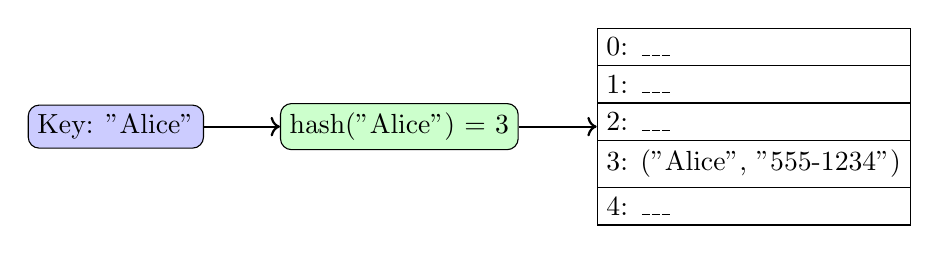
\begin{tikzpicture}[scale=0.9]
      \node[draw, rounded corners, fill=blue!20] (key) at (0,0) {Key: "Alice"};
      \node[draw, rounded corners, fill=green!20] (hash) at (4,0) {hash("Alice") = 3};
      \node[draw, rectangle split, rectangle split parts=5, rectangle split part align=left] (table) at (9,0) {
        \nodepart{one} 0: \_\_\_
        \nodepart{two} 1: \_\_\_
        \nodepart{three} 2: \_\_\_
        \nodepart{four} 3: ("Alice", "555-1234")
        \nodepart{five} 4: \_\_\_
      };

      \draw[->, thick] (key) -- (hash);
      \draw[->, thick] (hash) -- (table);
    \end{tikzpicture}
  \end{center}

  \vspace{0.3cm}
  \textbf{Performance:} Expected O(1) for insert, search, delete
\end{frame}

\begin{frame}{Why Use Hash Tables?}
  \textbf{Advantages:}
  \begin{itemize}
    \item \textbf{Fast lookups:} Average O(1) vs O(log n) for trees
    \item \textbf{Simple interface:} Natural key-value mapping
    \item \textbf{Flexible keys:} Strings, numbers, tuples, etc.
    \item \textbf{Widely used:} Python dicts, Java HashMap, C++ unordered\_map
  \end{itemize}

  \vspace{0.3cm}
  \textbf{Common Applications:}
  \begin{itemize}
    \item Dictionaries/maps (phone book, student records)
    \item Caching (LRU cache, memoization)
    \item Sets (unique element tracking)
    \item Frequency counting (word count)
    \item Database indexing
    \item Deduplication
  \end{itemize}
\end{frame}

\section{Hash Functions}

\begin{frame}{What Makes a Good Hash Function?}
  \textbf{Essential Properties:}
  \begin{enumerate}
    \item \textbf{Deterministic:} Same key always produces same hash
    \item \textbf{Uniform distribution:} Keys spread evenly across table
    \item \textbf{Fast to compute:} O(1) or O(k) where k = key length
    \item \textbf{Minimize collisions:} Different keys rarely map to same index
    \item \textbf{Avalanche effect:} Small key change → large hash change
  \end{enumerate}

  \vspace{0.3cm}
  \textbf{Hash Function Signature:}
  \begin{center}
    hash(key) $\rightarrow$ integer in range [0, table\_size - 1]
  \end{center}

  \vspace{0.3cm}
  \textbf{Goal:} Distribute keys uniformly to minimize collisions
\end{frame}

\begin{frame}[fragile]{Common Hash Functions: Division Method}
  \textbf{Simplest approach:} Use modulo operator

  \begin{lstlisting}[language=Python, basicstyle=\ttfamily\small]
def hash_division(key, table_size):
    return key % table_size
  \end{lstlisting}

  \vspace{0.3cm}
  \textbf{Example:}
  \begin{itemize}
    \item Key = 42, Table size = 13
    \item hash(42) = 42 \% 13 = 3
  \end{itemize}

  \vspace{0.3cm}
  \textbf{Best Practice:} Use prime table sizes
  \begin{itemize}
    \item Prime numbers: 53, 97, 193, 389, 769, 1543, ...
    \item Better distribution
    \item Fewer collisions
  \end{itemize}

  \vspace{0.3cm}
  \textbf{Trade-off:} Powers of 2 are faster (bitwise AND) but worse distribution
\end{frame}

\begin{frame}[fragile]{Common Hash Functions: Multiplication Method}
  \textbf{Idea:} Multiply by constant, extract fractional part

  \begin{lstlisting}[language=Python, basicstyle=\ttfamily\small]
def hash_multiplication(key, table_size):
    A = 0.6180339887  # (sqrt(5) - 1) / 2, golden ratio
    return int(table_size * ((key * A) % 1))
  \end{lstlisting}

  \vspace{0.3cm}
  \textbf{Advantages:}
  \begin{itemize}
    \item Works well with any table size
    \item Good distribution with golden ratio constant
    \item Independent of table size choice
  \end{itemize}

  \vspace{0.3cm}
  \textbf{Example:}
  \begin{itemize}
    \item Key = 123, A = 0.618, Table size = 100
    \item 123 $\times$ 0.618 = 76.014
    \item Fractional part: 0.014
    \item Index: $\lfloor$100 $\times$ 0.014$\rfloor$ = 1
  \end{itemize}
\end{frame}

\begin{frame}[fragile]{String Hashing: Polynomial Rolling Hash}
  \textbf{Challenge:} Hash strings efficiently

  \begin{lstlisting}[language=Python, basicstyle=\ttfamily\small]
def hash_string(s, table_size):
    hash_val = 0
    p = 31  # Prime base
    p_pow = 1

    for char in s:
        hash_val = (hash_val + ord(char) * p_pow) % table_size
        p_pow = (p_pow * p) % table_size

    return hash_val
  \end{lstlisting}

  \vspace{0.3cm}
  \textbf{Example: "hello"}
  \begin{itemize}
    \item h: 104 $\times$ 31$^0$
    \item e: 101 $\times$ 31$^1$
    \item l: 108 $\times$ 31$^2$
    \item l: 108 $\times$ 31$^3$
    \item o: 111 $\times$ 31$^4$
    \item Sum (mod table\_size) = hash value
  \end{itemize}

  \vspace{0.2cm}
  \textbf{Why prime base?} Better distribution, fewer collisions
\end{frame}

\begin{frame}[fragile]{Bad Hash Function Example}
  \textbf{What NOT to do:}

  \begin{lstlisting}[language=Python, basicstyle=\ttfamily\small]
# BAD: Only uses first character
def bad_hash(s, table_size):
    return ord(s[0]) % table_size
  \end{lstlisting}

  \vspace{0.3cm}
  \textbf{Problem:} Many collisions!
  \begin{itemize}
    \item "apple" $\rightarrow$ ord('a') = 97
    \item "ant" $\rightarrow$ ord('a') = 97
    \item "arrow" $\rightarrow$ ord('a') = 97
    \item All hash to same index!
  \end{itemize}

  \vspace{0.3cm}
  \textbf{Another bad example:}
  \begin{lstlisting}[language=Python, basicstyle=\ttfamily\small]
# BAD: All 5-letter words collide
def bad_hash2(s, table_size):
    return len(s) % table_size
  \end{lstlisting}

  \vspace{0.2cm}
  \textbf{Lesson:} Use all parts of the key for better distribution
\end{frame}

\section{Load Factor and Resizing}

\begin{frame}{Load Factor ($\alpha$)}
  \textbf{Definition:} $\alpha = \frac{n}{m}$ where
  \begin{itemize}
    \item n = number of elements
    \item m = table size
  \end{itemize}

  \vspace{0.3cm}
  \textbf{Meaning:} Average number of elements per slot

  \vspace{0.3cm}
  \textbf{Impact on Performance:}
  \begin{center}
    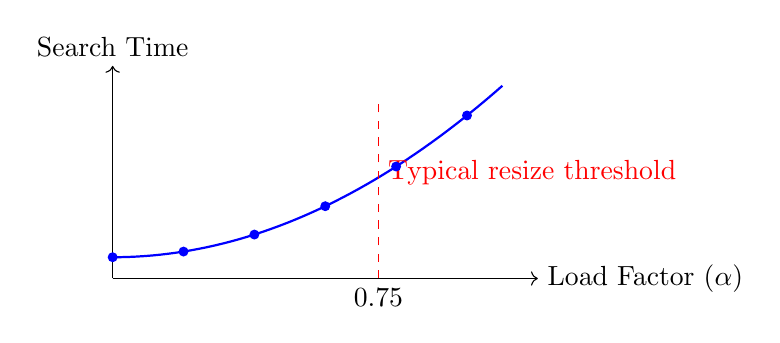
\begin{tikzpicture}[scale=0.9]
      \draw[->] (0,0) -- (6,0) node[right] {Load Factor ($\alpha$)};
      \draw[->] (0,0) -- (0,3) node[above] {Search Time};

      \draw[blue, thick, domain=0:5.5, samples=50] plot (\x, {0.3 + 0.8*\x*\x/10});

      \draw[dashed, red] (3.75,0) -- (3.75,2.5);
      \node[below] at (3.75,0) {0.75};
      \node[right, red] at (3.75,1.5) {Typical resize threshold};

      \fill[blue] (0,0.3) circle (2pt);
      \fill[blue] (1,0.38) circle (2pt);
      \fill[blue] (2,0.62) circle (2pt);
      \fill[blue] (3,1.02) circle (2pt);
      \fill[blue] (4,1.58) circle (2pt);
      \fill[blue] (5,2.3) circle (2pt);
    \end{tikzpicture}
  \end{center}

  \vspace{0.3cm}
  \textbf{Typical Thresholds:}
  \begin{itemize}
    \item \textbf{Chaining:} Resize when $\alpha > 0.75$ (Python uses 0.67)
    \item \textbf{Open addressing:} Resize when $\alpha > 0.5$
  \end{itemize}
\end{frame}

\begin{frame}[fragile]{Resizing Strategy}
  \begin{lstlisting}[language=Python, basicstyle=\ttfamily\footnotesize]
class HashTable:
    def __init__(self, initial_size=16):
        self.size = initial_size
        self.count = 0
        self.table = [[] for _ in range(self.size)]

    def load_factor(self):
        return self.count / self.size

    def resize(self):
        # Double the size
        old_table = self.table
        self.size *= 2
        self.table = [[] for _ in range(self.size)]
        self.count = 0

        # Rehash all elements
        for bucket in old_table:
            for key, value in bucket:
                self.insert(key, value)

    def insert(self, key, value):
        if self.load_factor() > 0.75:
            self.resize()

        index = hash(key) % self.size
        # Insert logic here
        self.count += 1
  \end{lstlisting}
\end{frame}

\begin{frame}{Amortized Analysis of Resizing}
  \textbf{Question:} Is resizing expensive?

  \vspace{0.3cm}
  \textbf{Analysis:}
  \begin{itemize}
    \item Insert n elements
    \item Resizes occur at: 1, 2, 4, 8, 16, ..., n
    \item Total rehashing cost: 1 + 2 + 4 + ... + n = 2n - 1 = O(n)
    \item Amortized cost per insertion: O(n) / n = \textbf{O(1)}
  \end{itemize}

  \vspace{0.3cm}
  \textbf{Visualization:}
  \begin{center}
    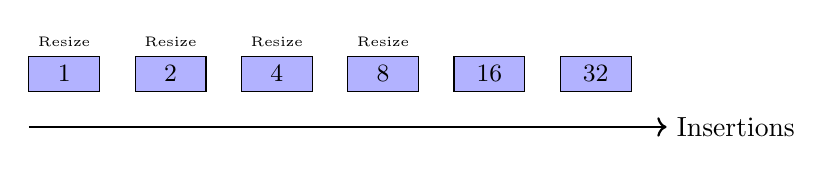
\begin{tikzpicture}[scale=0.9]
      \foreach \x/\n in {0/1, 1/2, 2/4, 3/8, 4/16, 5/32} {
        \draw[fill=blue!30] (\x*1.5,0) rectangle (\x*1.5+1,0.5);
        \node at (\x*1.5+0.5,0.25) {\small \n};
      }
      \draw[->, thick] (0,-0.5) -- (9,-0.5) node[right] {Insertions};
      \node[above] at (0.5,0.5) {\tiny Resize};
      \node[above] at (2,0.5) {\tiny Resize};
      \node[above] at (3.5,0.5) {\tiny Resize};
      \node[above] at (5,0.5) {\tiny Resize};
    \end{tikzpicture}
  \end{center}

  \vspace{0.3cm}
  \textbf{Key insight:} Expensive resizes are rare, so average cost is O(1)
\end{frame}

\section{Collision Handling}

\begin{frame}{Collision: When Two Keys Hash to Same Index}
  \textbf{Problem:} Different keys can hash to the same index

  \vspace{0.3cm}
  \begin{center}
    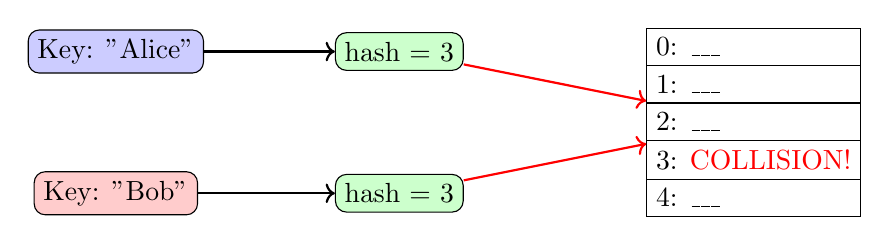
\begin{tikzpicture}[scale=0.9]
      \node[draw, rounded corners, fill=blue!20] (k1) at (0,1) {Key: "Alice"};
      \node[draw, rounded corners, fill=red!20] (k2) at (0,-1) {Key: "Bob"};

      \node[draw, rounded corners, fill=green!20] (h1) at (4,1) {hash = 3};
      \node[draw, rounded corners, fill=green!20] (h2) at (4,-1) {hash = 3};

      \node[draw, rectangle split, rectangle split parts=5, rectangle split part align=left] (table) at (9,0) {
        \nodepart{one} 0: \_\_\_
        \nodepart{two} 1: \_\_\_
        \nodepart{three} 2: \_\_\_
        \nodepart{four} 3: \textcolor{red}{COLLISION!}
        \nodepart{five} 4: \_\_\_
      };

      \draw[->, thick] (k1) -- (h1);
      \draw[->, thick] (k2) -- (h2);
      \draw[->, thick, red] (h1) -- (table);
      \draw[->, thick, red] (h2) -- (table);
    \end{tikzpicture}
  \end{center}

  \vspace{0.3cm}
  \textbf{Two Main Solutions:}
  \begin{enumerate}
    \item \textbf{Separate Chaining:} Store multiple elements at each index (linked list)
    \item \textbf{Open Addressing:} Find another empty slot in the table
  \end{enumerate}
\end{frame}

\begin{frame}{Separate Chaining}
  \textbf{Idea:} Each table slot stores a list of colliding elements

  \vspace{0.3cm}
  \begin{center}
    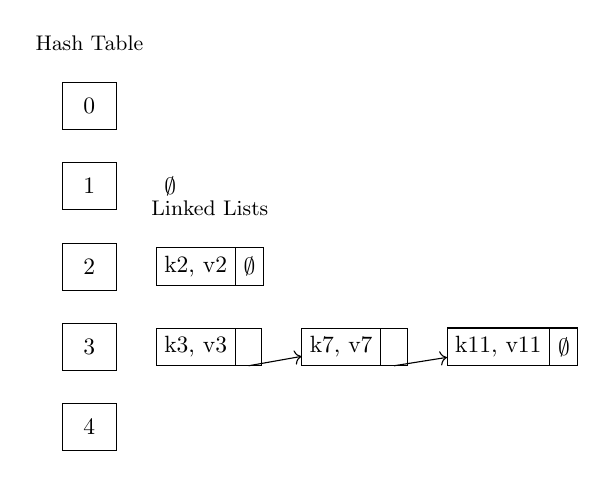
\begin{tikzpicture}[scale=0.85, every node/.style={scale=0.85}]
      \foreach \i in {0,1,2,3,4} {
        \node[draw, minimum width=0.8cm, minimum height=0.7cm] (slot\i) at (0,-\i*1.2) {\i};
      }

      % Slot 1: empty
      \node[right=0.5cm of slot1] {$\emptyset$};

      % Slot 2: one element
      \node[draw, rectangle split, rectangle split horizontal, rectangle split parts=2, right=0.5cm of slot2] (n2) {k2, v2 \nodepart{two} $\emptyset$};

      % Slot 3: three elements (collision chain)
      \node[draw, rectangle split, rectangle split horizontal, rectangle split parts=2, right=0.5cm of slot3] (n3a) {k3, v3 \nodepart{two}};
      \node[draw, rectangle split, rectangle split horizontal, rectangle split parts=2, right=0.5cm of n3a] (n3b) {k7, v7 \nodepart{two}};
      \node[draw, rectangle split, rectangle split horizontal, rectangle split parts=2, right=0.5cm of n3b] (n3c) {k11, v11 \nodepart{two} $\emptyset$};
      \draw[->] (n3a.two south) -- (n3b);
      \draw[->] (n3b.two south) -- (n3c);

      \node[above=0.3cm of slot0] {\small Hash Table};
      \node[above=0.3cm of n2] {\small Linked Lists};
    \end{tikzpicture}
  \end{center}

  \vspace{0.3cm}
  \textbf{Advantages:}
  \begin{itemize}
    \item Simple to implement
    \item Never fills up (can exceed load factor 1.0)
    \item Easy deletion
  \end{itemize}

  \textbf{Disadvantages:}
  \begin{itemize}
    \item Extra memory for pointers
    \item Poor cache locality
  \end{itemize}
\end{frame}

\begin{frame}[fragile]{Separate Chaining Implementation}
  \begin{lstlisting}[language=Python, basicstyle=\ttfamily\footnotesize]
class HashTableChaining:
    def __init__(self, size=10):
        self.size = size
        self.table = [[] for _ in range(size)]

    def insert(self, key, value):
        index = hash(key) % self.size
        bucket = self.table[index]

        # Update if key exists
        for i, (k, v) in enumerate(bucket):
            if k == key:
                bucket[i] = (key, value)
                return

        # Add new key-value pair
        bucket.append((key, value))

    def search(self, key):
        index = hash(key) % self.size
        bucket = self.table[index]

        for k, v in bucket:
            if k == key:
                return v

        return None  # Not found
  \end{lstlisting}
\end{frame}

\begin{frame}{Open Addressing}
  \textbf{Idea:} All elements stored in table, probe for empty slots

  \vspace{0.3cm}
  \begin{center}
    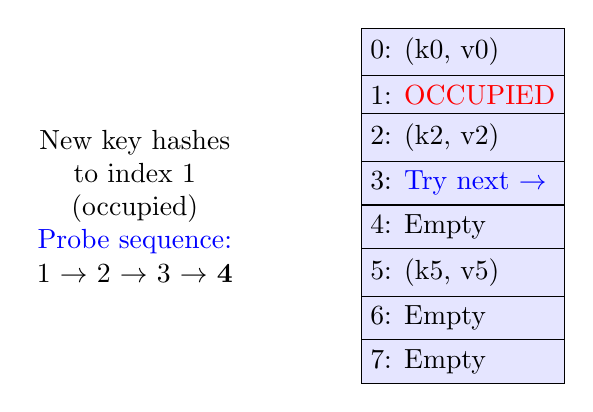
\begin{tikzpicture}[scale=0.9]
      \node[draw, rectangle split, rectangle split parts=8, rectangle split part align=left, fill=blue!10] (table) {
        \nodepart{one} 0: (k0, v0)
        \nodepart{two} 1: \textcolor{red}{OCCUPIED}
        \nodepart{three} 2: (k2, v2)
        \nodepart{four} 3: \textcolor{blue}{Try next $\rightarrow$}
        \nodepart{five} 4: Empty
        \nodepart{six} 5: (k5, v5)
        \nodepart{seven} 6: Empty
        \nodepart{eight} 7: Empty
      };

      \node[left=1.5cm of table, align=center] {
        New key hashes\\
        to index 1\\
        (occupied)\\
        \textcolor{blue}{Probe sequence:}\\
        1 $\rightarrow$ 2 $\rightarrow$ 3 $\rightarrow$ \textbf{4}
      };
    \end{tikzpicture}
  \end{center}

  \vspace{0.3cm}
  \textbf{Advantages:}
  \begin{itemize}
    \item Better cache locality
    \item No extra memory for pointers
  \end{itemize}

  \textbf{Disadvantages:}
  \begin{itemize}
    \item Must maintain low load factor ($< 0.7$)
    \item Complex deletion (need tombstones)
    \item Clustering issues
  \end{itemize}
\end{frame}

\begin{frame}{Comparison: Chaining vs Open Addressing}
  \begin{table}
    \centering
    \begin{tabular}{|l|c|c|}
      \hline
      \textbf{Feature} & \textbf{Chaining} & \textbf{Open Addressing} \\
      \hline
      Memory & More (pointers) & Less (no pointers) \\
      \hline
      Cache locality & Poor & Good \\
      \hline
      Load factor & Can exceed 1.0 & Must stay $< 0.7$ \\
      \hline
      Deletion & Simple & Complex (tombstones) \\
      \hline
      Clustering & No & Yes \\
      \hline
      Implementation & Easier & Harder \\
      \hline
      Best for & General use & Cache-friendly, known size \\
      \hline
    \end{tabular}
  \end{table}

  \vspace{0.5cm}
  \textbf{Recommendation:}
  \begin{itemize}
    \item Use chaining for most applications (simpler, more flexible)
    \item Use open addressing for performance-critical, cache-sensitive code
  \end{itemize}
\end{frame}

\section{Open Addressing Strategies}

\begin{frame}{Linear Probing}
  \textbf{Formula:} h(k, i) = (h(k) + i) \% m

  \textbf{Probe sequence:} h(k), h(k)+1, h(k)+2, h(k)+3, ...

  \vspace{0.3cm}
  \textbf{Example:} Key hashes to index 3, table size = 10
  \begin{center}
    Probe: 3 $\rightarrow$ 4 $\rightarrow$ 5 $\rightarrow$ 6 $\rightarrow$ 7 $\rightarrow$ 8 $\rightarrow$ 9 $\rightarrow$ 0 $\rightarrow$ 1 $\rightarrow$ 2
  \end{center}

  \vspace{0.3cm}
  \textbf{Advantages:}
  \begin{itemize}
    \item Simple to implement
    \item Good cache locality (sequential access)
  \end{itemize}

  \textbf{Disadvantages:}
  \begin{itemize}
    \item \textbf{Primary clustering:} Long runs of occupied slots form
  \end{itemize}

  \vspace{0.3cm}
  \textbf{Clustering Example:}
  \begin{center}
    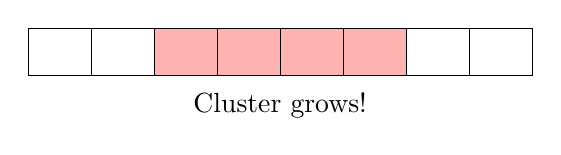
\begin{tikzpicture}[scale=0.8]
      \foreach \i/\c in {0/white, 1/white, 2/red!30, 3/red!30, 4/red!30, 5/red!30, 6/white, 7/white} {
        \node[draw, fill=\c, minimum width=0.8cm, minimum height=0.6cm] at (\i,0) {};
      }
      \node[below] at (3.5,-0.5) {Cluster grows!};
    \end{tikzpicture}
  \end{center}
\end{frame}

\begin{frame}{Quadratic Probing}
  \textbf{Formula:} h(k, i) = (h(k) + i²) \% m

  \textbf{Probe sequence:} h(k), h(k)+1, h(k)+4, h(k)+9, h(k)+16, ...

  \vspace{0.3cm}
  \textbf{Example:} Key hashes to index 3, table size = 10
  \begin{center}
    \begin{tabular}{c|c|c}
      i & Offset & Index \\
      \hline
      0 & 0 & 3 \\
      1 & 1 & 4 \\
      2 & 4 & 7 \\
      3 & 9 & 2 \\
      4 & 16 & 9 \\
    \end{tabular}
  \end{center}

  \vspace{0.3cm}
  \textbf{Advantages:}
  \begin{itemize}
    \item Reduces primary clustering
    \item Better distribution than linear
  \end{itemize}

  \textbf{Disadvantages:}
  \begin{itemize}
    \item \textbf{Secondary clustering:} Keys with same hash follow same probe sequence
    \item May not probe all slots (need prime table size)
  \end{itemize}
\end{frame}

\begin{frame}{Double Hashing}
  \textbf{Formula:} h(k, i) = ($h_1$(k) + i $\times$ $h_2$(k)) \% m

  \textbf{Two hash functions:}
  \begin{itemize}
    \item $h_1$(k): Initial position
    \item $h_2$(k): Step size (must be coprime with m)
  \end{itemize}

  \vspace{0.3cm}
  \textbf{Example:} $h_1$(k) = 3, $h_2$(k) = 7, table size = 10
  \begin{center}
    \begin{tabular}{c|c|c}
      i & Offset & Index \\
      \hline
      0 & 0 & 3 \\
      1 & 7 & 0 \\
      2 & 14 & 7 \\
      3 & 21 & 4 \\
      4 & 28 & 1 \\
    \end{tabular}
  \end{center}

  \vspace{0.3cm}
  \textbf{Advantages:}
  \begin{itemize}
    \item Eliminates both primary and secondary clustering
    \item Best distribution among open addressing methods
  \end{itemize}

  \textbf{Disadvantages:}
  \begin{itemize}
    \item More complex to implement
    \item Two hash function computations
  \end{itemize}
\end{frame}

\begin{frame}{Comparison of Probing Methods}
  \begin{table}
    \centering
    \begin{tabular}{|l|c|c|c|}
      \hline
      \textbf{Method} & \textbf{Clustering} & \textbf{Complexity} & \textbf{Distribution} \\
      \hline
      Linear & Primary & Simple & Poor \\
      \hline
      Quadratic & Secondary & Moderate & Good \\
      \hline
      Double Hashing & None & Complex & Excellent \\
      \hline
    \end{tabular}
  \end{table}

  \vspace{0.5cm}
  \textbf{Clustering Visualization:}
  \begin{center}
    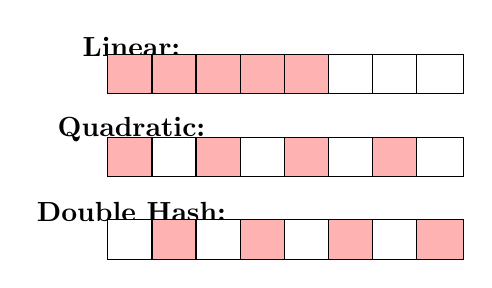
\begin{tikzpicture}[scale=0.7]
      \node[align=left] at (0,2) {\textbf{Linear:}};
      \foreach \i/\c in {0/red!30, 1/red!30, 2/red!30, 3/red!30, 4/red!30, 5/white, 6/white, 7/white} {
        \node[draw, fill=\c, minimum width=0.6cm, minimum height=0.5cm] at (\i*0.8,1.5) {};
      }

      \node[align=left] at (0,0.5) {\textbf{Quadratic:}};
      \foreach \i/\c in {0/red!30, 1/white, 2/red!30, 3/white, 4/red!30, 5/white, 6/red!30, 7/white} {
        \node[draw, fill=\c, minimum width=0.6cm, minimum height=0.5cm] at (\i*0.8,0) {};
      }

      \node[align=left] at (0,-1) {\textbf{Double Hash:}};
      \foreach \i/\c in {0/white, 1/red!30, 2/white, 3/red!30, 4/white, 5/red!30, 6/white, 7/red!30} {
        \node[draw, fill=\c, minimum width=0.6cm, minimum height=0.5cm] at (\i*0.8,-1.5) {};
      }
    \end{tikzpicture}
  \end{center}
\end{frame}

\section{Deletion in Open Addressing}

\begin{frame}{The Deletion Problem}
  \textbf{Challenge:} Cannot simply set slot to None

  \vspace{0.3cm}
  \textbf{Example Problem:}
  \begin{enumerate}
    \item Insert k1 at index 1, k2 at index 2 (k2 collided, probed to 2)
    \item Delete k1 (set index 1 to None)
    \item Search for k2:
      \begin{itemize}
        \item Start at index 1
        \item Find None $\rightarrow$ stop searching
        \item k2 is "lost" even though it's at index 2!
      \end{itemize}
  \end{enumerate}

  \vspace{0.3cm}
  \begin{center}
    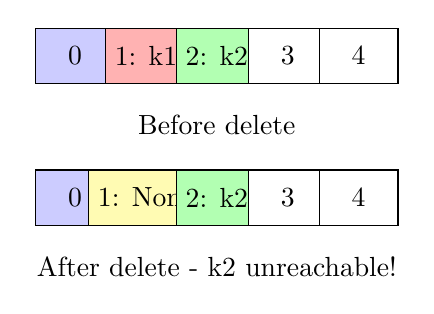
\begin{tikzpicture}[scale=0.9]
      \foreach \i/\c/\t in {0/blue!20/0, 1/red!30/1: k1, 2/green!30/2: k2, 3/white/3, 4/white/4} {
        \node[draw, fill=\c, minimum width=1cm, minimum height=0.7cm] at (\i,0) {\t};
      }
      \node[below] at (2,-0.7) {Before delete};

      \foreach \i/\c/\t in {0/blue!20/0, 1/yellow!30/1: None, 2/green!30/2: k2, 3/white/3, 4/white/4} {
        \node[draw, fill=\c, minimum width=1cm, minimum height=0.7cm] at (\i,-2) {\t};
      }
      \node[below] at (2,-2.7) {After delete - k2 unreachable!};
    \end{tikzpicture}
  \end{center}
\end{frame}

\begin{frame}{Solution: Tombstones (Lazy Deletion)}
  \textbf{Idea:} Mark deleted slots with special DELETED marker

  \vspace{0.3cm}
  \textbf{Rules:}
  \begin{itemize}
    \item \textbf{Insert:} Can place at None or DELETED slots
    \item \textbf{Search:} Skip over DELETED, continue probing
    \item \textbf{Delete:} Mark slot as DELETED (not None)
  \end{itemize}

  \vspace{0.3cm}
  \begin{center}
    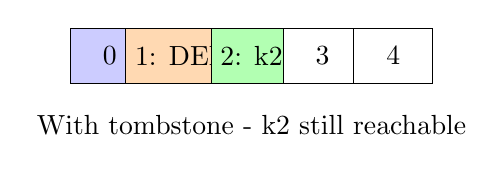
\begin{tikzpicture}[scale=0.9]
      \foreach \i/\c/\t in {0/blue!20/0, 1/orange!30/1: DEL, 2/green!30/2: k2, 3/white/3, 4/white/4} {
        \node[draw, fill=\c, minimum width=1cm, minimum height=0.7cm] at (\i,0) {\t};
      }
      \node[below] at (2,-0.7) {With tombstone - k2 still reachable};
    \end{tikzpicture}
  \end{center}

  \vspace{0.3cm}
  \textbf{Tombstone Issues:}
  \begin{itemize}
    \item DELETED markers accumulate over time
    \item Degrade search performance
    \item Waste space
  \end{itemize}

  \vspace{0.3cm}
  \textbf{Solution:} Rehash when too many tombstones (e.g., > 25\% of table)
\end{frame}

\begin{frame}[fragile]{Deletion Implementation}
  \begin{lstlisting}[language=Python, basicstyle=\ttfamily\footnotesize]
class HashTableWithDeletion:
    DELETED = object()  # Sentinel value

    def delete(self, key):
        for i in range(self.size):
            index = (hash(key) + i) % self.size

            if self.table[index] is None:
                return False  # Not found

            if self.table[index] is not self.DELETED:
                if self.table[index][0] == key:
                    self.table[index] = self.DELETED
                    return True

        return False

    def search(self, key):
        for i in range(self.size):
            index = (hash(key) + i) % self.size

            if self.table[index] is None:
                return None  # Not found

            # Skip DELETED, continue probing
            if self.table[index] is not self.DELETED:
                if self.table[index][0] == key:
                    return self.table[index][1]

        return None
  \end{lstlisting}
\end{frame}

\section{Applications}

\begin{frame}[fragile]{Application: Dictionaries / Maps}
  \textbf{Most common use case:} Key-value storage

  \begin{lstlisting}[language=Python, basicstyle=\ttfamily\small]
# Python dict (hash table implementation)
phonebook = {
    "Alice": "555-1234",
    "Bob": "555-5678",
    "Charlie": "555-9012"
}

# O(1) average case operations
phone = phonebook["Alice"]  # Lookup
phonebook["David"] = "555-3456"  # Insert
del phonebook["Bob"]  # Delete
exists = "Charlie" in phonebook  # Membership test
  \end{lstlisting}

  \vspace{0.3cm}
  \textbf{Real-world examples:}
  \begin{itemize}
    \item Student records (ID $\rightarrow$ student info)
    \item Configuration files (setting name $\rightarrow$ value)
    \item Symbol tables (variable name $\rightarrow$ value)
  \end{itemize}
\end{frame}

\begin{frame}[fragile]{Application: Caching (LRU Cache)}
  \begin{lstlisting}[language=Python, basicstyle=\ttfamily\footnotesize]
from collections import OrderedDict

class LRUCache:
    def __init__(self, capacity):
        self.cache = OrderedDict()
        self.capacity = capacity

    def get(self, key):
        if key not in self.cache:
            return -1
        # Move to end (most recently used)
        self.cache.move_to_end(key)
        return self.cache[key]

    def put(self, key, value):
        if key in self.cache:
            self.cache.move_to_end(key)
        self.cache[key] = value
        if len(self.cache) > self.capacity:
            # Remove least recently used (first item)
            self.cache.popitem(last=False)

# Example usage
cache = LRUCache(2)
cache.put(1, "A")
cache.put(2, "B")
cache.get(1)       # Returns "A", moves 1 to end
cache.put(3, "C")  # Evicts key 2 (least recently used)
  \end{lstlisting}
\end{frame}

\begin{frame}[fragile]{Application: Frequency Counting}
  \begin{lstlisting}[language=Python, basicstyle=\ttfamily\small]
from collections import Counter

# Count word frequencies
text = "the quick brown fox jumps over the lazy dog"
word_count = Counter(text.split())
print(word_count)
# Counter({'the': 2, 'quick': 1, 'brown': 1, 'fox': 1, ...})

# Most common words
print(word_count.most_common(3))
# [('the', 2), ('quick', 1), ('brown', 1)]

# Manual implementation
def count_frequencies(items):
    freq = {}
    for item in items:
        freq[item] = freq.get(item, 0) + 1
    return freq
  \end{lstlisting}

  \vspace{0.3cm}
  \textbf{Applications:}
  \begin{itemize}
    \item Text analysis (word frequency)
    \item Log analysis (error frequency)
    \item User behavior (page visit counts)
  \end{itemize}
\end{frame}

\begin{frame}[fragile]{Application: Two Sum Problem}
  \textbf{Problem:} Find two numbers that sum to target

  \begin{lstlisting}[language=Python, basicstyle=\ttfamily\small]
def two_sum(nums, target):
    """
    Given array and target, return indices of two numbers
    that add up to target.

    Time: O(n), Space: O(n)
    """
    seen = {}
    for i, num in enumerate(nums):
        complement = target - num
        if complement in seen:
            return [seen[complement], i]
        seen[num] = i
    return None

# Example
nums = [2, 7, 11, 15]
target = 9
print(two_sum(nums, target))  # [0, 1] (2 + 7 = 9)
  \end{lstlisting}

  \vspace{0.3cm}
  \textbf{Key insight:} Hash table enables O(1) lookup of complement
\end{frame}

\begin{frame}[fragile]{Application: Deduplication}
  \begin{lstlisting}[language=Python, basicstyle=\ttfamily\small]
def remove_duplicates(arr):
    """Remove duplicates while preserving order"""
    seen = set()
    result = []
    for item in arr:
        if item not in seen:
            seen.add(item)
            result.append(item)
    return result

# Example
arr = [1, 2, 3, 2, 4, 1, 5]
print(remove_duplicates(arr))
# [1, 2, 3, 4, 5]

# Using set (loses order)
unique = list(set(arr))
# [1, 2, 3, 4, 5] (order not guaranteed)
  \end{lstlisting}

  \vspace{0.3cm}
  \textbf{Applications:}
  \begin{itemize}
    \item Remove duplicate emails from mailing list
    \item Find unique visitors to website
    \item Detect duplicate transactions
  \end{itemize}
\end{frame}

\section{Complexity and Pitfalls}

\begin{frame}{Time Complexity}
  \begin{table}
    \centering
    \begin{tabular}{|l|c|c|c|}
      \hline
      \textbf{Operation} & \textbf{Average} & \textbf{Worst} & \textbf{Notes} \\
      \hline
      Insert & O(1) & O(n) & Worst: all keys collide \\
      \hline
      Search & O(1) & O(n) & Worst: all keys collide \\
      \hline
      Delete & O(1) & O(n) & Worst: all keys collide \\
      \hline
      Resize & O(n) & O(n) & Amortized O(1) per insert \\
      \hline
    \end{tabular}
  \end{table}

  \vspace{0.5cm}
  \textbf{Space Complexity:}
  \begin{itemize}
    \item \textbf{Chaining:} O(n + m) where n = elements, m = table size
    \item \textbf{Open addressing:} O(m), must keep load factor low
  \end{itemize}

  \vspace{0.3cm}
  \textbf{Key Point:} Expected O(1) depends on:
  \begin{itemize}
    \item Good hash function (uniform distribution)
    \item Reasonable load factor ($< 0.75$)
    \item Proper collision handling
  \end{itemize}
\end{frame}

\begin{frame}[fragile]{Common Pitfall 1: Mutable Keys}
  \textbf{Problem:} Using mutable objects as keys

  \begin{lstlisting}[language=Python, basicstyle=\ttfamily\small]
# BAD: Lists are mutable, can't be hashed
d = {[1, 2]: "value"}  # TypeError: unhashable type: 'list'

# BAD: Dictionaries are mutable
d = {{1: 2}: "value"}  # TypeError: unhashable type: 'dict'

# GOOD: Use immutable types
d = {(1, 2): "value"}              # Tuples work
d = {frozenset([1, 2]): "value"}   # Frozen sets work
d = {"key": "value"}               # Strings work
d = {42: "value"}                  # Integers work
  \end{lstlisting}

  \vspace{0.3cm}
  \textbf{Rule:} Keys must be immutable and hashable
  \begin{itemize}
    \item \textbf{Hashable:} int, float, str, tuple, frozenset
    \item \textbf{Not hashable:} list, dict, set
  \end{itemize}
\end{frame}

\begin{frame}[fragile]{Common Pitfall 2: Poor Hash Function}
  \begin{lstlisting}[language=Python, basicstyle=\ttfamily\small]
# BAD: All strings of same length collide
def bad_hash(s):
    return len(s) % 10

# All 5-letter words map to index 5!
# "hello", "world", "apple" -> all collide

# BAD: Only uses first character
def bad_hash2(s):
    return ord(s[0]) % 10

# "ant", "apple", "arrow" -> all collide
  \end{lstlisting}

  \vspace{0.3cm}
  \textbf{Consequences:}
  \begin{itemize}
    \item Many collisions
    \item Performance degrades to O(n)
    \item Long collision chains
  \end{itemize}

  \vspace{0.3cm}
  \textbf{Solution:} Use all parts of key, use proven hash functions
\end{frame}

\begin{frame}[fragile]{Common Pitfall 3: Ignoring Load Factor}
  \begin{lstlisting}[language=Python, basicstyle=\ttfamily\small]
# BAD: Never resize
class BadHashTable:
    def __init__(self):
        self.table = [[] for _ in range(10)]
        # Fixed size!

    def insert(self, key, value):
        index = hash(key) % 10
        self.table[index].append((key, value))
        # Just keep inserting...
        # Performance degrades to O(n)!
  \end{lstlisting}

  \vspace{0.3cm}
  \textbf{Problem:} With 1000 elements in size-10 table:
  \begin{itemize}
    \item Load factor = 100
    \item Average chain length = 100
    \item Search time = O(100) = O(n)
  \end{itemize}

  \vspace{0.3cm}
  \textbf{Solution:} Monitor load factor, resize when needed
\end{frame}

\begin{frame}{When NOT to Use Hash Tables}
  \textbf{Hash tables are NOT suitable when you need:}

  \vspace{0.3cm}
  \begin{itemize}
    \item \textbf{Ordered iteration:} Use BST or sorted array
      \begin{itemize}
        \item Hash tables don't maintain order
      \end{itemize}

    \vspace{0.2cm}
    \item \textbf{Range queries:} Use BST or B-tree
      \begin{itemize}
        \item "Find all keys between 10 and 20"
      \end{itemize}

    \vspace{0.2cm}
    \item \textbf{Minimum/maximum:} Use heap
      \begin{itemize}
        \item Hash tables need O(n) to find min/max
      \end{itemize}

    \vspace{0.2cm}
    \item \textbf{Worst-case guarantees:} Use balanced trees
      \begin{itemize}
        \item Hash tables can degrade to O(n)
      \end{itemize}

    \vspace{0.2cm}
    \item \textbf{Memory constrained:} Consider alternatives
      \begin{itemize}
        \item Hash tables waste space (load factor $< 1$)
      \end{itemize}
  \end{itemize}
\end{frame}

\section{Summary}

\begin{frame}{Key Concepts Recap}
  \textbf{Hash Table Fundamentals:}
  \begin{itemize}
    \item Hash function maps keys to array indices
    \item Expected O(1) insert, search, delete
    \item Trade space for time
  \end{itemize}

  \vspace{0.3cm}
  \textbf{Good Hash Function:}
  \begin{itemize}
    \item Deterministic, uniform, fast
    \item Minimize collisions
    \item Common methods: division, multiplication, polynomial
  \end{itemize}

  \vspace{0.3cm}
  \textbf{Load Factor Management:}
  \begin{itemize}
    \item $\alpha = n / m$ (elements / table size)
    \item Resize when $\alpha > 0.75$ (chaining) or $\alpha > 0.5$ (open addressing)
    \item Amortized O(1) resizing cost
  \end{itemize}
\end{frame}

\begin{frame}{Collision Handling Recap}
  \textbf{Separate Chaining:}
  \begin{itemize}
    \item Store lists at each index
    \item Simple, never fills up
    \item Extra memory, poor cache locality
  \end{itemize}

  \vspace{0.3cm}
  \textbf{Open Addressing:}
  \begin{itemize}
    \item Probe for next empty slot
    \item Better cache locality, no pointers
    \item Complex deletion (tombstones)
    \item Three methods:
      \begin{itemize}
        \item Linear probing (simple, primary clustering)
        \item Quadratic probing (better, secondary clustering)
        \item Double hashing (best, no clustering)
      \end{itemize}
  \end{itemize}
\end{frame}

\begin{frame}{Applications Recap}
  \textbf{Common Uses:}
  \begin{itemize}
    \item Dictionaries/maps (key-value storage)
    \item Caching (LRU cache)
    \item Sets (unique elements)
    \item Frequency counting
    \item Database indexing
    \item Deduplication
    \item Two sum and related problems
  \end{itemize}

  \vspace{0.3cm}
  \textbf{Best Practices:}
  \begin{itemize}
    \item Use immutable keys only
    \item Choose good hash function
    \item Monitor and maintain load factor
    \item Resize when needed
    \item Use chaining for most cases
  \end{itemize}
\end{frame}

\begin{frame}{Practice Problems}
  \textbf{Basic:}
  \begin{itemize}
    \item Implement hash table with chaining
    \item Implement hash table with linear probing
    \item Design hash function for strings
  \end{itemize}

  \vspace{0.3cm}
  \textbf{Intermediate:}
  \begin{itemize}
    \item LRU Cache (LeetCode 146)
    \item Two Sum (LeetCode 1)
    \item Group Anagrams (LeetCode 49)
    \item First Unique Character (LeetCode 387)
    \item Implement resizing with load factor
  \end{itemize}

  \vspace{0.3cm}
  \textbf{Advanced:}
  \begin{itemize}
    \item Design hashmap with all operations (LeetCode 706)
    \item LFU Cache (LeetCode 460)
    \item Implement quadratic probing
    \item Implement double hashing
    \item Analyze hash function quality
  \end{itemize}
\end{frame}

\begin{frame}{Further Learning}
  \textbf{Advanced Topics:}
  \begin{itemize}
    \item Universal hashing families
    \item Perfect hashing
    \item Cuckoo hashing
    \item Robin Hood hashing
    \item Bloom filters (probabilistic hash structures)
  \end{itemize}

  \vspace{0.3cm}
  \textbf{Resources:}
  \begin{itemize}
    \item CLRS: Chapter 11 (Hash Tables)
    \item Practice on LeetCode hash table tag
    \item Study Python dict implementation (CPython source)
    \item Analyze hash functions with test data
  \end{itemize}

  \vspace{0.3cm}
  \textbf{Projects:}
  \begin{itemize}
    \item Build your own hash table library
    \item Implement LRU cache from scratch
    \item Create spell checker with hash table
    \item Design in-memory database with hash indexing
  \end{itemize}
\end{frame}

\begin{frame}
  \begin{center}
    {\Huge Thank You!}

    \vspace{1cm}
    {\Large Questions?}

    \vspace{1cm}
    \textbf{Hash Tables: Fast Average-Case Performance}
  \end{center}
\end{frame}

\end{document}
